\chapter{ Proposed Solution}


In there paper by (Kaiping Xue, Senior Member, IEEE,), they proposed a new scheme to enable ABE to implement comparable attributes, called Comparable Attribute-based Encryption (CABE). In CABE, we  use a unique way to generate and manage sub-attributes for comparable attributes, so as to make a solution for addressing the above issue in an efficient way, in terms of both storage overhead and computation overhead. Our solution in dealing with sub-attributes are based on a special notion called 0-encoding and 1-encoding. The main contributions of this paper can be summarized as follows:
\begin{enumerate}
    \item We propose an efficient method based on a special concept 0-encoding and 1-encoding, so that the attributes can be used in arbitrary comparison, which is suitable for ABE system;
     \item A lightweight and efficient CABE construction is proposed. This construction halves the expanded storage overhead in average compared with related schemes, and significantly decreases the computation overhead in encryption and decryption from O(log n) to O(1) (N denotes the value space of the attribute dimension).
\end{enumerate}
\textbf{
\section{Definition of 0-Encoding and 1-Encoding}
}
Our system uses the concept of two special encodings, 0-encoding and 1-encoding.
Let 
\[{s = s_ns_{n-1} \ldots s_1 \in \{0,1\}^n}\]

 be an n-length binary string of a value for a certain attribute dimension. 

\begin{itemize}
    \item The 0-encoding of s is defined as a set such that \[{ S^0_s\ = \{ {s}_ns_{n-1} \ldots s_{i+1}1|s_i = 0,1<=i<=n \} } \]
     \item The 1-encoding of s is defined as a set such that \[{ S^0_s\ = \{ {s}_ns_{n-1} \ldots s_{i}|s_i = 1,1<=i<=n \} } \]
\end{itemize}
Intuitively, 1-encoding of s is the set of all its odd prefix substrings, and the 0-encoding is the set of all of its modified even prefix substrings, where the least significant bit is flipped from “0” to “1”. The size of set S0s equals to the number of characters “0” in string s, and meanwhile the size of S1s equals to the number of “1”. 
Compared with the value space of n-length binary string: N=2n, both S1s and S0s have at most log N elements. To compare two integers x and y in the form of n-length binary string, we encode x into 1-encoding  and into 0-encoding \(S_0^y\)  . We make the judgment that \[ x > y \] if and only if there’s an element in both \(S_1^x\) and \(S_0^y\)  . A formula to express this theorem is as

\begin{figure}[h]
    \centering
    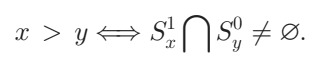
\includegraphics[width=0.3\linewidth]{Images/IntersectionOfSets.jpeg}
   
\end{figure}

\begin{figure}[h]
    \centering
    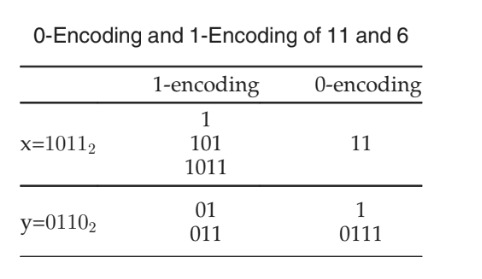
\includegraphics[width=0.7\linewidth]{Images/01EncodingTable.jpeg}
   
\end{figure}

\textbf{
\section{Storing of 0-Encoding and 1-Encoding}
}
The object we deal with is such an attribute that is not an exact value, but stands as a range of continuous values, and may be matched in comparison in the ABE system, such as “\(Score > 75\)”, “\(Age < 25\)”. For one attribute field F, whose value space is N and minimum value is \(val_{min}\), we can reduce the storage overhead to ½(\(log_2N)\) on average to make this kind of attribute suit  CP-ABE construction with utilization of 0-encoding and 1-encoding. Our procedure is implemented as follows  For a value x  F, if its minimum value is not zero, compute 
\(x_m\)=x - \(val_{min}\);
otherwise, such operations can be skipped. For clarity of description, let \(x_m\)=x; in this case. If the length of the binary string \(x_m\) is less than \(log_2N\), use 0 to fill at high bits. Then what the program deals with is a new \(log_2N\)-long binary string \(x_m\). We encode \(x_m\) into 0-encoding \(S_0\)
\(x_m\) and 1-encoding S1 \(x_m\) with the rule described in Section 3.1. For a certain access structure, if the access policy needs the corresponding attribute F to satisfy that \(F > x\), an attribute set \(Set_{c0}\)(F,x) can be designed as . A formula to express this theorem is as

\begin{figure}[h]
    \centering
    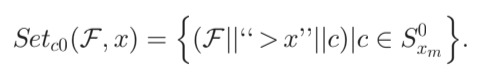
\includegraphics[width=0.6\linewidth]{Images/ConcatenationOfConditions.jpeg}
   
\end{figure}

\begin{figure}[h]
    \centering
    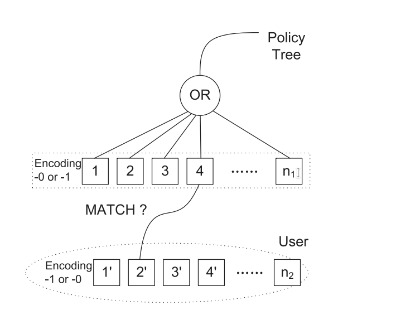
\includegraphics[width=0.7\linewidth]{Images/TreeOrMatching.jpeg}
   
\end{figure}



\textbf{
\section{Proposed Range Query Solution}
}
Since we already exposed the mathematical construct on how to reduce the numerical comparison to simple binary AND and OR operations we will now propose our solution for efficient range query. Some lemmas must be mentioned before proposing our solution : 
\begin{itemize}
    \item \textbf{
    Lemma 1 : Encode a into its 0-Encoding set  \(E_0\) and b into its 1-encoding set \(E_1\) , we have \(b > a\) if and only if \(E_1\) and \(E_0\) have some elements in common.
    }
    \item From this lemma we can derive the theorem that the common element will be a single element.
    A further observation that can be made from this is that if there is no common element between the 2 sets then \(b<=a\). 

\end{itemize}
Now in our solution we decided to perform some operations on the access policy with the range comparisons such that the intersection of the 2 0-Encoding and 1-Encoding set can be left up to the access policy tree itself and it will perform the intersection on the elements in 2 sets using the binary operations. This is done using the logic that say we want to find the intersection between 2 sets say set A and set B then if say we have 1 encoding of set A , the individual elements of 1 - encoding of the set can be taken in the form A1 OR A2 OR A3 OR A4 which are nothing but the individual elements of the 1-encoding. 

Now say we get an actual value to compare then we can calculate it’s 0-encoding and push that itself in the access tree and tell our access tree to perform the intersection function by doing comparison of individual elements thus resulting in intersection of the 2 sets of 1- Encoding of A and 0-Encoding of B and if access tree returns 1 that is true then it has found an element in intersection and thus we have successfully calculated that \(b < a\).

Similarly we can swap the encoding schemes for integers and get the result 
 “ \(x > value\) “ 
Now to implement the negation comparison for an attribute like “ \(x!= value\)  ” we decided to do a deep dive in boolean logic along with set theory and for the given conditions we came up with the solution that if “ \(x < value or x > value \) ” returns a 0 value that means \(x != value\) . Proof for this lies in the fact that if \(x == value \)then \(x < value\) returns None and \(x > value\) returns None and if we take \(None OR None\) we get\(None\)  aka \(0 aka False\). Now any number except value can be \(either >\) value or \(< value\) where the condition “ \( x < value or x > value \) ” will return true hence the negation condition can be implemented successfully. So we were able to implement range based comparison by combining the 2 conditions like “\(x < a and x > b \)“ such that “\(x belongs to ( b,a )\)”  and “ \(x<a or x >a \)” implying “ \(x!=a\) ”.

Hence we were able to efficiently implement range based comparison in the access tree compared to previously known inefficient method which basically involved iterating through all the numbers in a given range \(( 1,n )\) such that it performed equality check on all individual numbers in the given range thus becoming increasingly inefficient when the range of numbers became very big as inherent complexity of that is \(O(n)\) in both time as well as more complexity in space due to overhead of maintaining the access structure as well.


In our proposed solution and implementation we have cut down the time complexity from \(O (N)\) to \(O (log N)\)  and space complexity to \(O (log N)\) as well, which we will demonstrate via some benchmarking graphs that we calculated on our code.







